\documentclass{article}
\usepackage[utf8]{inputenc}
\usepackage{listings}
\usepackage{indentfirst}
\title{HW4for590}
\author{hesong huang,yuan feng  }
\date{April 2018}

\usepackage{natbib}
\usepackage{graphicx}

\begin{document}

\maketitle

\section{Introduction}
(1) Database design

In our implementation, we designed three tables to store account information, positions and orders:
\begin{figure}[h!]
\centering
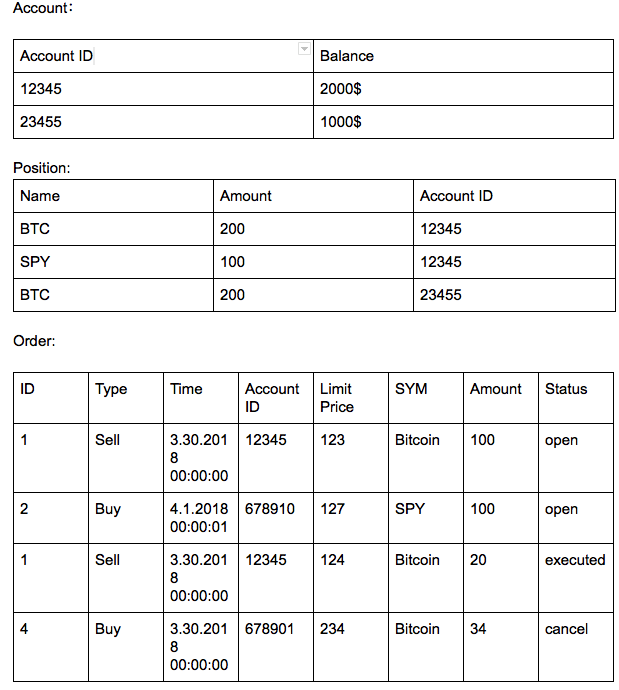
\includegraphics[scale=0.45]{Snip3}
\caption{Three database tables}
\label{fig:Snip3}
\end{figure}

(2) XML parsing

In this project, we utilized RapidXml, parsing strings into a DOM Trees. As it is parsing, we called the functions simultaneously, and write results in a DOM Tree. And we send back the DOM Tree to the client as strings in the formate of XML.


\section{Methods to improve scalability}

(1) Block and Unblock Socket

We choose block module to receive xml requests. 

If we block socket when receiving request, program would wait until a new request arrives. If we use the unblock method using select function to receive request, the select function would wait for specific seconds. If no request arrive during this period, select function would return and the program would keep moving on. However, in this project, using block and non block methods have tiny influence on scalability, because the main job of our program is to wait for the coming request and create a new thread to handle that request. So in our main function, the program do nothing but wait for request. \\

(2) Mutex Lock and Database Lock

In this program, race condition may happen when different threads. For example, two buy requests may match the same sell order.  

We tried two methods to prevent race condition. One is adding mutex between each transaction. The other is using postgres row lock. With this row lock, when one thread is reading and editing a row in a table, the other thread cannot read and edit this row. Finally, we chose to use database row low.\\

(3) Index 

We created three tables using postgresql: account, position and order.
Index in database is used for speed up the performance of queries. In our program, we add index for each table:
ACCOUNT(ACCOUNT ID);
POSITION(ACCOUNT ID,SYMBOL);
ORDERS(TYPE,STATUS,SYMBOL);



 
\section{Test cases} 
We sent lots of xml files a time to our server using .sh. Following are the some of the xml we select to represent the test cases. Test cases are divided in two parts:
\begin{enumerate}
 \item Test cases:
   \begin{enumerate}
   \item Create account  and symbol requests:  
      \begin{lstlisting}
161                                                                     <?xml version=1.0 encoding=UTF-8?>
<create>
  <account id="26" balance="1000"/>
  <symbol sym="SYM26">
    <account id="26">1000</account>
  </symbol>
</create>

      \end{lstlisting}
      \item Transaction requests:  
      \begin{lstlisting}

230                                                                     <?xml version=1.0 encoding=UTF-8?>
<transactions accountid="1">
  <order sym="SYM1" amount="-500" limit="11"></order>
</transactions>
<transactions accountid="1">
  <order sym="SYM0" amount="50" limit="20"></order>
</transactions>

      \end{lstlisting}
      
       \item Cancel requests:  
      \begin{lstlisting}

140
<?xml version=1.0 encoding=UTF-8?>
<transactions accountid="12334">
  <cancel uid="2" ></cancel>
  <cancel uid="9" ></cancel>
</transactions>
      \end{lstlisting}
      
      \item Query requests:  
      \begin{lstlisting}
135                                                                     <?xml version=1.0 encoding=UTF-8?>
<transactions accountid="1">
  <query uid="1" ></query>
  <query uid="2" ></query>
</transactions>
      \end{lstlisting}
   \end{enumerate}
 \item Results:
     \begin{enumerate}
     \item Created
     \begin{lstlisting}
<?xml version="1.0" encoding="UTF-8"?>
<results>
  <created ID="26"/>
  <created ID="26" SYM="SYM26"/>
</results>
     \end{lstlisting}
      
      
     \item Opened
     \begin{lstlisting}
<?xml version="1.0" encoding="UTF-8"?>
<results>
  <opened SYM="SYM1" amount="-500" limit="11" uid="9"/>
</results>
<results>
  <opened SYM="SYM0" amount="50" limit="20" uid="10"/>
</results>
     \end{lstlisting}
     
     \item Canceled
     \begin{lstlisting}
     <?xml version="1.0" encoding="UTF-8"?>
<results>
	<canceled>
		<canceled shares="50" time="1523054343.09397"/>
	</canceled>
	<canceled>
		<canceled shares="500" time="1523054343.16968"/>
	</canceled>
</results>
     \end{lstlisting}
     
     \item Query
     \begin{lstlisting}
<?xml version="1.0" encoding="UTF-8"?>
<results>
  <status>
    <open shares="450"/>
    <executed shares="50" price="11" time="1523054086.92808"/>
  </status>
  <status>
    <canceled shares="50" time="1523054343.09397"/>
  </status>
</results>
     \end{lstlisting}
      \end{enumerate}
      
\end{enumerate}

\section{Scalability}
To test scalability, we need to compare the running time of serialization method and parallel method. We send a bunch of xml files at a time to our server. We increase the number of xml files from one to one thousand, and the execution time is shown in following table. this table only shows the execution time of parallel method: 

\begin{figure}[h!]
\centering
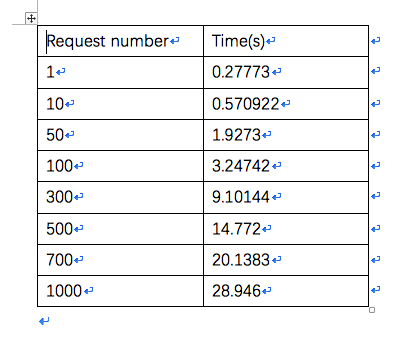
\includegraphics[scale=0.5]{Snip2}
\caption{Request number and whole executed time}
\label{fig:Snip2}
\end{figure}

As we can see in these figures, parallel method increased the scalability of program. As the request number increases, the capability to improve scalability tends to be a stable value.

\begin{figure}[h!]
\centering
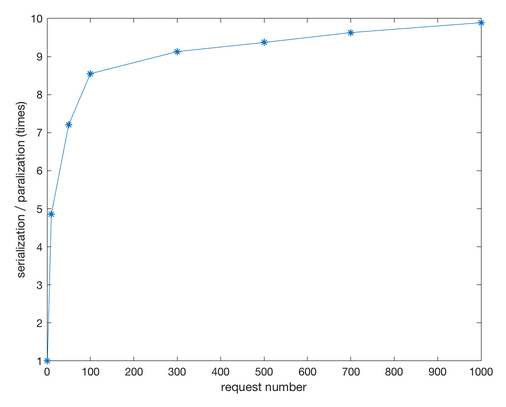
\includegraphics[scale=0.5]{Snip}
\caption{ use serialization method / use parallel method }
\label{fig:Snip}
\end{figure}





\end{document}
